%\begin{figure}[h!]
%	\centering
%	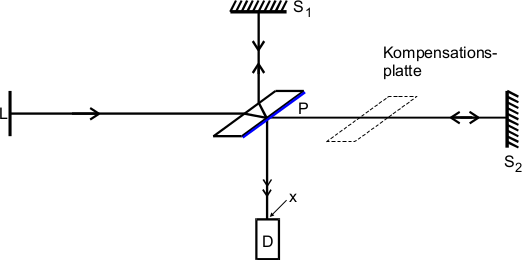
\includegraphics[width=0.7\textwidth]{Interferometer.png}
%	\caption{Versuchsaufbau, der eine nicht interferenzfähige Lichtquelle für Interferenz-Experimente erlaubt}
%	\label{Gluhlampe}
%\end{figure}
\begin{center}
	\begin{tikzpicture}
	\node(LASER)at(-6,0)[rectangle,draw]{Laser};
	\node(center)at(0,0){};
	\node(S1)at(6,0){};
	\node(S2)at(0,4){};
	\node(D)at(0,-4)[rectangle,draw]{Photodiode};

%Beschriftung	
	\node(hdl)at(-2,-1.5){semipermeabler Spiegel};
	\node(Box)at(-2,2.5){Messbox};.5
	\node(K)at(3,-1){Kompensationsplatte};
	\node(Spiegel2)at(2,4){S2};
	\node(Spiegel1)at(6,1.5){S1};
	
	\path [-]
	(-1,-1)edge(1,1)            % semipermeabler Spiegel
	(LASER)edge(S1)             % Strahlengang
	(S2)edge(D)                 % Strahlengang
	(-1.5,3.85)edge(1.5,3.85)   % Spiegel 2
	(5.85,-1)edge(5.85,1);      % Spiegel 1	
	\end{tikzpicture}
\end{center}
Zentraler Bestandteil des Versuchs ist ein Michelson-Interferometer (siehe Abbildung VERWEIS). Es ist ein kreuzförmiger Aufbau, bei dem sich jeweils ein Spiegel (S1) und ein Laser und ein zweiter Spiegel (S2) und ein Photodetektor gegenüber stehen. In der Mitte befindet sich ein semipermeabler Spiegel (SP). \\
Beim Einschalten des Lasers bewegt sich der Lichtstrahl auf SP zu. Dort wird er geteilt. Die beiden einzelnen Strahlen laufen auf S1 oder S2 zu und werden dort reflektiert. Jeder dieser Strahlen wird bei SP abermals geteilt und so treffen zwei parallele Lichtstrahlen auf die Photodiode und erzeugen ein Interferenzbild. Die Intensität im Zentrum wird durch \eqref{Intensitat}
\begin{align}
	I = 2\vec{E}_0^2\left(1+\cos\Delta s\right) \ ,
\end{align}
mit dem Wegunterschied
\begin{align}
	\Delta s = 2(\overline{SPS1}-\overline{SPS2}) \ ,
\end{align}
beschrieben.